\documentclass[dvipsnames,beamer]{standalone}

\usepackage{textcomp}
\usepackage{lmodern}

\usepackage{tikz}
\usetikzlibrary{positioning,decorations.pathreplacing,fit}
\usetikzlibrary{decorations.markings,arrows.meta,shapes.arrows,arrows}
\usetikzlibrary{calc}

\definecolor{mygreen}{RGB}{0,128,80}
\colorlet{darkgreen}{mygreen!90!black}


\begin{document}

%\small

\begin{standaloneframe}


\resizebox{\textwidth}{!}{

\begin{tikzpicture}[
	>=triangle 60,
	arrow double line/.style={
		double distance = 20pt,
   		shorten <= 11.5, 	
   		shorten >= 16.1,
   		very thick,
	    postaction = {
    		draw = white,
	 	    line width = 20pt,
	 	    shorten <=-.1pt,
	 	    shorten >=-.1pt,	
	    },
	    postaction = {
	    	decorate, 
	    	decoration = {
	    		markings, 
	    		mark=at position 0 with {
	    			\arrow[xshift=26.6pt]{Straight Barb[reversed,length=-1pt 0.7]}
	    		},
	    		mark = at position 1 with {
   	    			\arrow[xshift=10.6pt]{Straight Barb[length=-1pt 0.7]}
   	    		}
	    	}
	    }
	},
	fat arrow double line/.style={
		double distance = 23pt,
   		shorten <= 12.5, 	
   		shorten >= 17.5,
   		very thick,
		 postaction = {
		   		draw = white,
		  line width = 23pt,
		  shorten <=-.1pt,
		  shorten >=-.1pt,	
		 },
		 postaction = {
	    	decorate, 
	    	decoration = {
	    		markings, 
	    		mark=at position 0 with {
	    			\arrow[xshift=29.4pt]{Straight Barb[reversed,length=-3pt 0.75]}
	    		},
	    		mark = at position 1 with {
	  	    			\arrow[xshift=12.6pt]{Straight Barb[length=-3pt 0.75]}
	  	    		}
	    	}
 		}
	},
	mysingle/.style = {
		double distance = 22,
		shorten <= 10.5, 	
		shorten >= 14,
		very thick,
		postaction = {
	 		draw = white,
			line width = 22pt,
			shorten <=8pt,
			shorten >=-.5pt,	
		},
		postaction = {
			decorate, 
			decoration = {
				markings, 
				mark = at position 1 with {
					\arrow [xshift=15]{Straight Barb[length=15]}
				}
			}
		},	
	},
	mybrace/.style= {
		decorate, decoration={brace,amplitude=5pt,raise=5pt}, thick
	},
	comment box/.style = {
		draw,inner sep = 6pt,fill=gray!25,thick,rounded corners=3pt,text=black,font=\large
	},
	every node/.style={
		font=\bfseries\boldmath
	},	
	]

	

		
	\node[] (client) {Client};
	\node[right = 4.3 of client] (AP) {{\alt<3,7-9>{\textcolor{lightgray!25}{Access point}}{Access point}}};
	\node[right = 4.0 of  AP] (AS) {{\alt<4>{\textcolor{lightgray!25}{Server}}{Server}}};
	\def\InterMsgSpaceVertical{1.2}
	

	\node[inner sep=0pt, xshift=0cm,yshift=0.8cm] (laptop_icon) at (client) {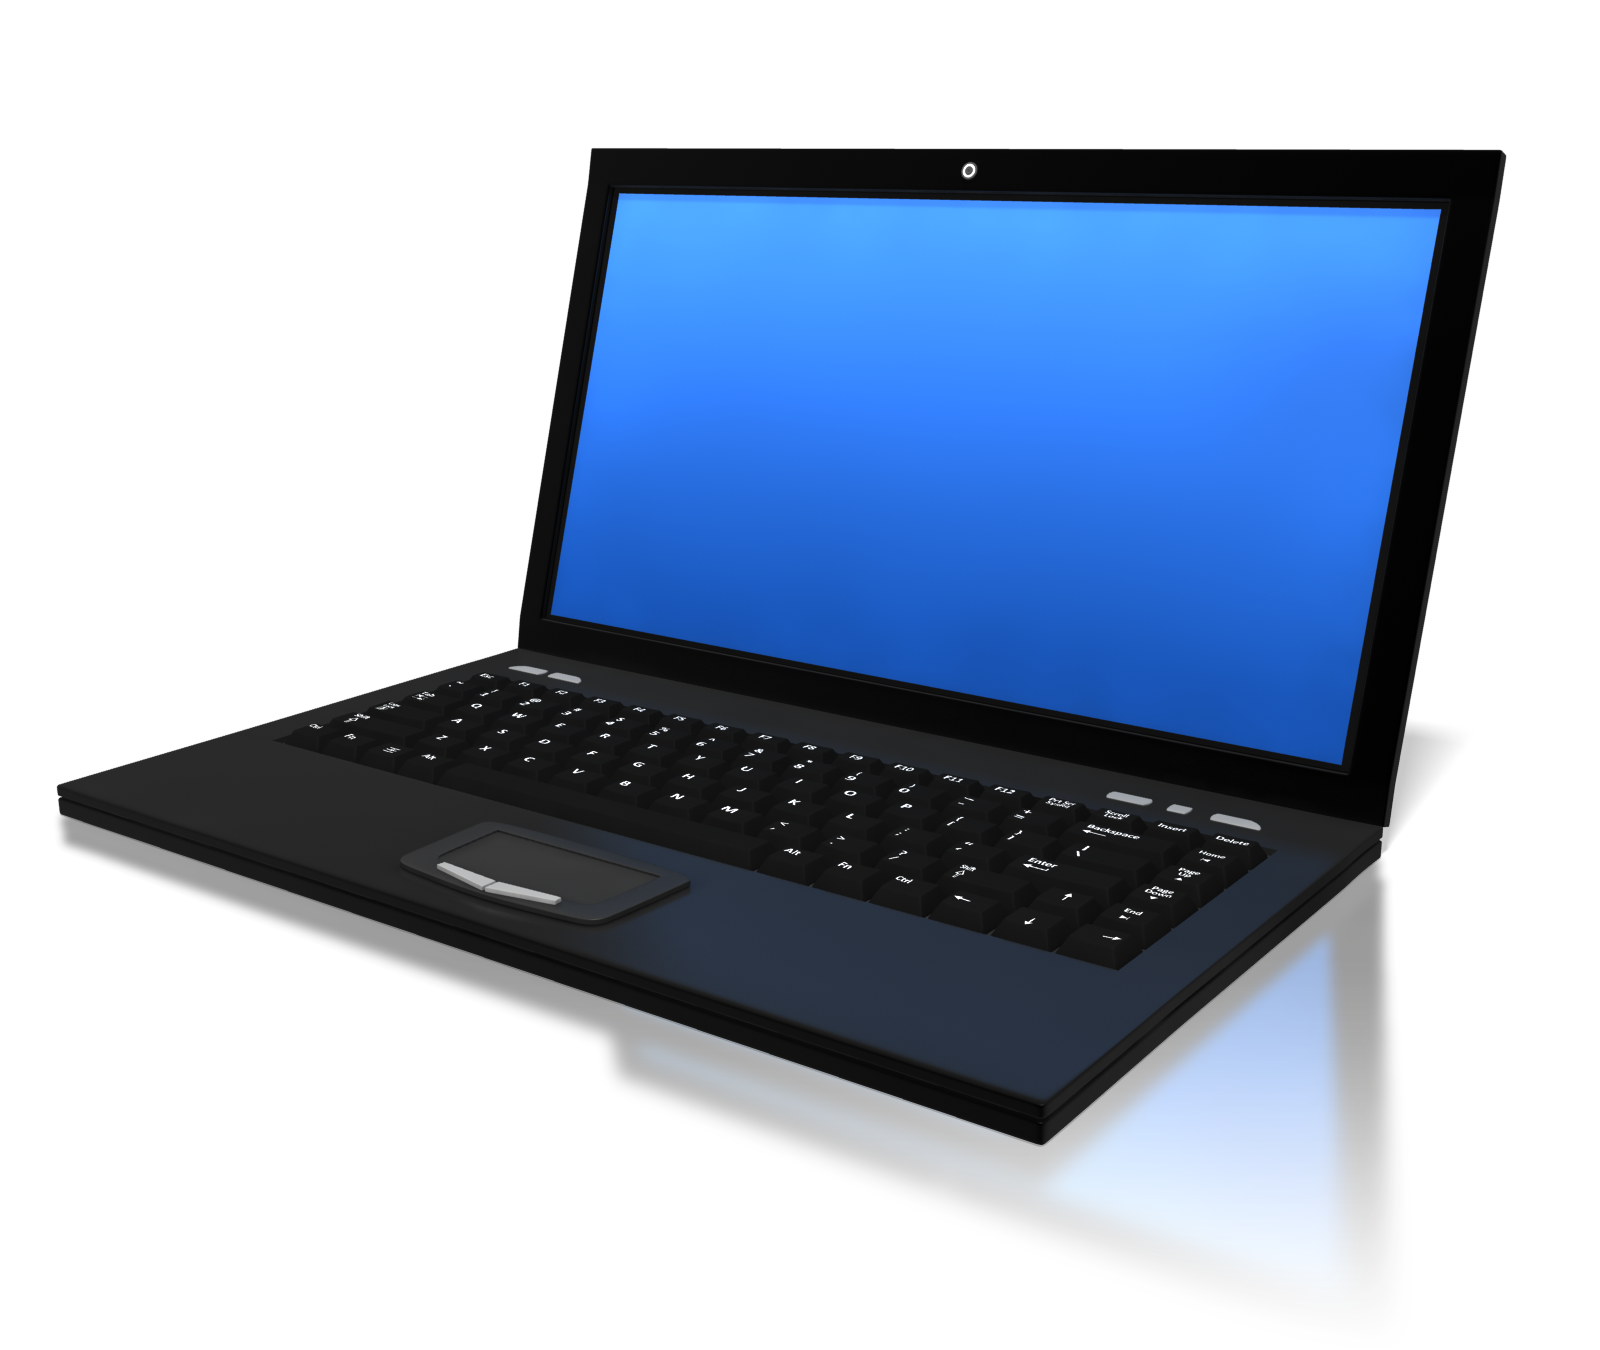
\includegraphics[width=.15\textwidth]{laptop}};
	
	\node[inner sep=0pt, xshift=-0.0cm,yshift=1.1cm] (AP_icon) at (AP) {
		{\alt<3,7-9>{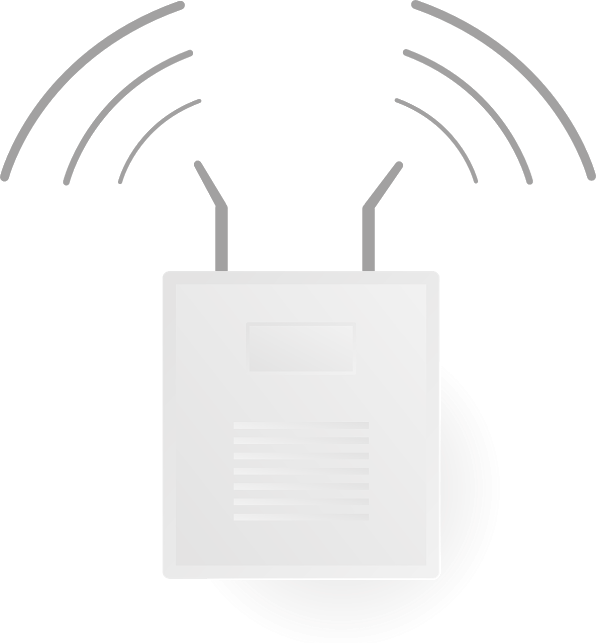
\includegraphics[width=.13\textwidth]{AP_grey}}
			{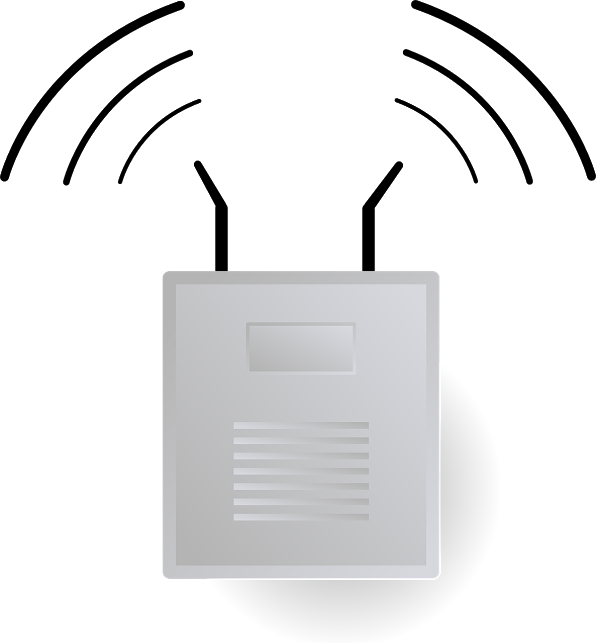
\includegraphics[width=.13\textwidth]{AP}}
		}
	};

	\node[above = -0.2 of AS] (server_icon) {
		{\alt<4>{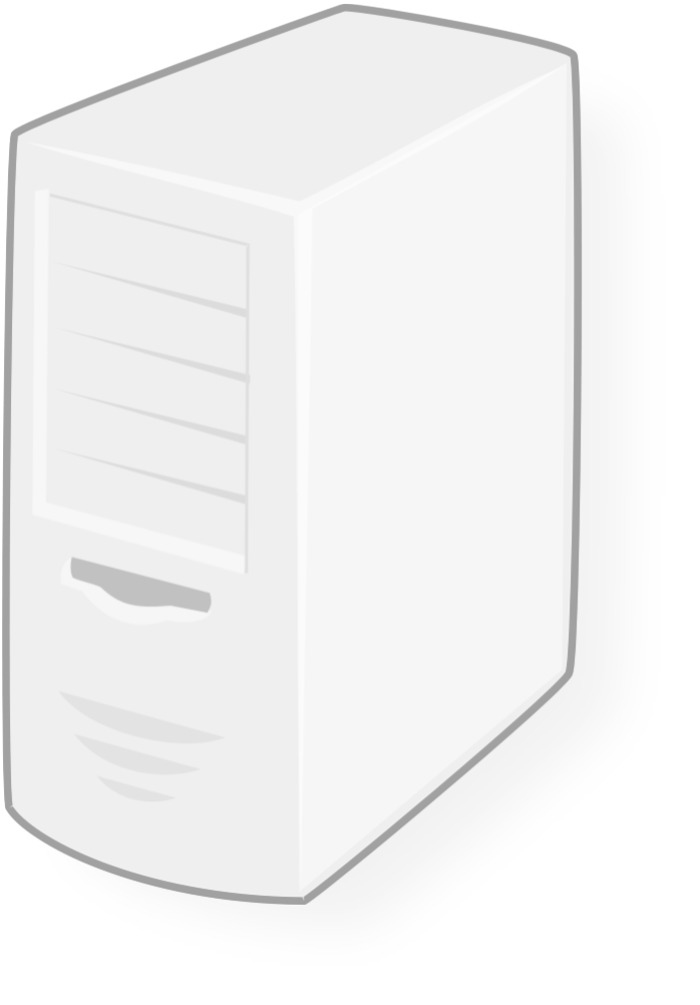
\includegraphics[width=.1\textwidth]{server_gray}}
			{
\includegraphics[width=.1\textwidth]{server}}
		}
	};

	
	\foreach \i in {1,...,4} {
		\coordinate[below = \InterMsgSpaceVertical * \i of client] (c\i) {};
		\coordinate[below = \InterMsgSpaceVertical * \i of AP] (ap\i) {};
		\coordinate[below = \InterMsgSpaceVertical * \i of AS] (as\i) {};
	}
	
	
	\visible<1-2,6,7>{
		\draw[arrow double line,red] (c1) -- node (EAP) {EAP method} (as1);
	}
	
	\visible<1-2,5>{
		\draw[arrow double line,blue] (ap2) -- node[xshift=-2,blue] (AAA) {Key transport} (as2);
		\draw[mybrace] ([yshift=15]as1) -- node[right=0.4,align=center] (3P-KD) {EAP} ([yshift=-15]as2);
	}
	
	
	\visible<3,5,8>{
		\draw[arrow double line,red] (c1) -- node (EAP) {EAP-TLS} (as1);
	}
	
	\visible<2,4-6>{
		\draw[arrow double line,darkgreen] (c3) -- node[xshift=-2] {\alt<2,6>{Key confirmation}{IEEE 802.11}} (ap3);
	}


	\visible<5>{
		\draw[mybrace, decoration={mirror}, left] ([xshift=-4,yshift=15]c1) -- node[left=0.4,align=center] {WPA2\\Enterprise} ([xshift=-4,yshift=-15]c3);
	}
	
	\visible<6>{%
		\draw[fat arrow double line, Plum] (c1) -- node[xshift=5pt] {EAP} (as1);
		\draw[mysingle, Plum] ([yshift=-1]ap1) --  ([yshift=-4]ap2);
	}	
	
	
	\visible<8-9>{
		\node[inner sep=0pt, xshift=0.75cm,yshift=0.75cm] (client_cert) at (laptop_icon) {
\includegraphics[width=.1\textwidth]{cert}};
		\node[inner sep=0pt, xshift=0.3cm,yshift=0.7cm] (server_cert) at (server_icon) {
\includegraphics[width=.1\textwidth]{cert}};
	}
	
	\visible<9>{
		\draw[double,double distance=26,shorten >= 0.95cm, shorten <= 0.8cm, ultra thick, red,
				postaction = {
					draw = white,
					line width = 26pt,
					shorten <= -.1pt,
					shorten >= -.1pt,	
				}
		] (c1) -- (as1);
	
		\draw[arrow double line] (c1) -- node (tls) {TLS} (as1);
		\node[above= 0.2cm of tls,red]  {EAP packets};
		
		
		\node[left = 0.1cm of c1] {
			
\includegraphics[width=.06\textwidth,trim=0 7cm 0 4cm]{key_orange}	
		};
		
		\node[right = -0.1cm of as1] {
			
\includegraphics[width=.06\textwidth,trim=0 7cm 0 4cm]{key_orange}	
		};
		
		\node[draw, inner sep=8pt,thick,fill=lightgray!2] at (ap3) {
			
\includegraphics[width=.06\textwidth,trim=0 7cm 0 4cm]{key_red} $\gets \mathbf{KDF}(
					
\includegraphics[width=.06\textwidth,trim=0 7cm 0 4cm]{key_orange}, ``\mathtt{EAP-TLS}")$
		};
	}
		

\end{tikzpicture}
}

\end{standaloneframe}

\end{document}